\documentclass[11pt,a4paper]{article}
\usepackage[margin=24mm]{geometry}
\usepackage[T1]{fontenc}
\usepackage{lmodern,microtype,amsmath,amssymb,amsthm,mathtools,booktabs,array,longtable,graphicx}
\usepackage[hidelinks]{hyperref}
\usepackage{xcolor,fancyhdr}
\hypersetup{pdftitle={Exact conditional contraction for Pauli channels and depolarization in every dimension},pdfauthor={Dev D. Goyal},pdfsubject={Exact channel coefficients with Lean 4 verification},pdfkeywords={quantum information, conditional contraction, depolarization, Pauli channels, Lean 4}}
\definecolor{ink}{HTML}{17334D}
\pagestyle{fancy}\fancyhf{}\fancyhead[L]{\small Exact conditional quantum contraction}
\fancyhead[R]{\small Quantum information}\fancyfoot[C]{\thepage}
\setlength{\headheight}{14pt}\setlength{\parskip}{4pt}
\newtheorem{theorem}{Theorem}
\newtheorem{lemma}[theorem]{Lemma}
\newtheorem{proposition}[theorem]{Proposition}
\newtheorem{corollary}[theorem]{Corollary}
\newcommand{\Tr}{\operatorname{Tr}}
\newcommand{\id}{\operatorname{id}}
\newcommand{\cN}{\mathcal N}
\newcommand{\cD}{\mathcal D}
\newcommand{\cP}{\mathcal P}
\newcommand{\cE}{\mathcal E}
\newcommand{\norm}[1]{\left\lVert#1\right\rVert}
\newcommand{\ket}[1]{\lvert#1\rangle}
\newcommand{\bra}[1]{\langle#1\rvert}
\newcommand{\psd}{\succeq0}
\newcommand{\etal}{\eta^{\Delta}_{E_\gamma}}
\newcommand{\etatr}{\eta^{\Delta}_T}
\newcommand{\etac}{\eta^{c}_T}
\title{\vspace{-1cm}\color{ink}\textbf{Exact conditional contraction for Pauli channels\\and depolarization in every dimension}}
\author{Dev D. Goyal}
\date{29 October 2026}
\begin{document}\maketitle
\noindent\textbf{Autonomous AI research disclosure.} The research, proofs, manuscript and formalization were produced through fully autonomous agentic AI research. Dev D. Goyal is responsible for publication. No expert human validation or external peer review is claimed.\par\medskip
\begin{abstract}
This paper determines the conditional trace-distance contraction coefficient of every stochastic Pauli qubit channel and of the full physical depolarizing family in every dimension. If $a,b$ are the two smallest Pauli probabilities, the answer is $1-8ab/(a+b)$, with value one when both vanish. For $d\ge2$ and negative depolarization $\cN_s(X)=(1+s)\Tr(X)I_d/d-sX$, $0\le s\le1/(d^2-1)$, the answer is $s[1+(d^2-1)s]/[1-(d^2-3)s]$. The positive-multiplier branch has its standard value $\lambda$. All conditional hockey-stick parameters $\gamma\ge1$ have these same values. The negative-parameter upper bound holds for every Hermitian input with every finite quantum reference; a balanced tight frame encoded in a genuine Bell basis supplies matching normalized density witnesses. An explicit nonlinear decomposition of binary effects proves the upper without asserting a physical degrading channel. The resulting sharp binary-comparison threshold can be of order $d^{-2}$ while the physical erasure-simulation threshold remains constant. Priority is not certified, and the paper has not been externally peer reviewed. The final verification status is recorded in Section~\ref{sec:formal}.
\end{abstract}

\section{The research problem and its scope}
The quantity studied here measures how much distinguishability survives a channel after the distinguishability already present in a retained quantum reference is subtracted. Its optimization includes unequal reference marginals and arbitrarily large finite references. Computing an ordinary trace contraction coefficient, or imposing equal reference marginals, does not solve this optimization.

The framework and general positive-Doeblin upper bound are established in Hirche, George, Nuradha and Wilde~\cite{Conditional}, building on the quantum Doeblin theory of George, Hirche, Nuradha and Wilde~\cite{Doeblin}. The present problem is quantitative: determine the exact coefficient, with an unrestricted upper bound and matching actual states, for the entire Pauli family and for depolarization in every dimension. Theorems below give full parameter ranges, all ties and boundary cases, rather than a numerical estimate or a selected special parameter.

The proof combines a reference-flag identity, a sharp qubit effect bound and an all-dimensional matching lower witness with its arbitrary-effect upper bound. Harmonic interpolation, Bell bases, standard qubit channel normal forms and the cited support-vector constructions are credited ingredients.

\section{Definitions and exact statements}
Let $\cN:A\to B$ be a finite-dimensional CPTP map and $\cN_R=\id_R\otimes\cN$. For density operators define
\[
 T(\rho,\sigma)=\tfrac12\norm{\rho-\sigma}_1,\qquad
 E_\gamma(\rho\Vert\sigma)=\Tr(\rho-\gamma\sigma)_+,\qquad \gamma\ge1.
\]
Write $\rho_R=\Tr_A\rho$ and
\[
 \Delta_\gamma(\rho,\sigma)=E_\gamma(\rho\Vert\sigma)-E_\gamma(\rho_R\Vert\sigma_R).
\]
The coefficient is the literal supremum
\begin{equation}\label{eq:definition}
 \etal(\cN)=\sup_{\substack{R,\rho,\sigma\\\Delta_\gamma(\rho,\sigma)>0}}
 \frac{\Delta_\gamma(\cN_R\rho,\cN_R\sigma)}{\Delta_\gamma(\rho,\sigma)}.
\end{equation}
All finite $R$ and all PSD trace-one input states are admitted. At $\gamma=1$ this is $\etatr$. For comparison,
\[
 \etac(\cN)=\sup_{\substack{R,\rho,\sigma:\rho_R=\sigma_R\\T(\rho,\sigma)>0}}
 \frac{T(\cN_R\rho,\cN_R\sigma)}{T(\rho,\sigma)}.
\]
The positive Doeblin coefficient uses the unnormalized Choi matrix $J_{\cN}$:
\[
 \alpha_+(\cN)=\sup\{\Tr P:P\psd,\ J_{\cN}\succeq I_A\otimes P\}.
\]
For Hermitian $X$ set $X_R=\Tr_A X$ and
\begin{equation}\label{eq:gap}
 g(X)=\Tr X_+-\Tr(X_R)_+=\tfrac12(\norm X_1-\norm{X_R}_1).
\end{equation}
Thus $\Delta_\gamma(\rho,\sigma)=g(\rho-\gamma\sigma)$. A channel preserves $X_R$, a fact used explicitly in the formal development.

\begin{theorem}[Every Pauli channel]\label{thm:pauli}
Let $w_0,w_1,w_2,w_3\ge0$ sum to one and
\[
 \cP_w(X)=\sum_{j=0}^3 w_j\sigma_jX\sigma_j^\dagger,
 \qquad (\sigma_0,\sigma_1,\sigma_2,\sigma_3)=(I,X,Y,Z).
\]
Let $a\le b$ be the two smallest weights, counted with multiplicity. For every $\gamma\ge1$,
\begin{equation}\label{eq:pauli}
 \etal(\cP_w)=\etatr(\cP_w)=1-\frac{8ab}{a+b}.
\end{equation}
If $a=b=0$, the right side means one. The positive Doeblin coefficient is $4a$.
\end{theorem}

The deficit in~\eqref{eq:pauli} is the harmonic mean of $4a$ and $4b$. The standard unitary normal form for unital qubit channels~\cite[Theorem 2.2]{ChoiLi}, together with invariance under input and output unitary conjugations, gives the corresponding mathematical formula for every unital qubit channel. In terms of the two least eigenvalues $\mu_1,\mu_2$ of its \emph{unnormalized} Choi matrix, it is $1-4\mu_1\mu_2/(\mu_1+\mu_2)$. The supplied Lean theorem directly covers all stochastic Pauli channels; normal-form existence itself is not encoded in this project.

\begin{theorem}[Depolarization in every dimension]\label{thm:depol}
For $d\ge2$ let
\[
 \mathcal D_\lambda(X)=\lambda X+(1-\lambda)\Tr(X)I_d/d,
 \qquad -\frac1{d^2-1}\le\lambda\le1.
\]
For every $\gamma\ge1$,
\begin{equation}\label{eq:full-depol}
 \etal(\mathcal D_\lambda)=\etatr(\mathcal D_\lambda)=
 \begin{cases}
 \lambda,&0\le\lambda\le1,\\[2mm]
 \displaystyle\frac{s[1+(d^2-1)s]}{1-(d^2-3)s},
 &\lambda=-s,\quad0\le s\le1/(d^2-1).
 \end{cases}
\end{equation}
For the negative branch, put $n=d^2$ and $p_n(s)=s[1+(n-1)s]/[1-(n-3)s]$. Then
\[
 \etac(\cN_s)=s,\qquad \alpha_+(\cN_s)=1-(n-1)s.
\]
In the strict physical interior,
\[
 s<p_n(s)<(n-1)s.
\]
\end{theorem}

The denominator is positive throughout the closed interval: it equals
$1-(n-1)s+2s$, and at the upper endpoint it is $2/(n-1)$. The formal negative-branch theorem uses the explicit canonical $d$-dimensional basis indexed by $\mathbb Z/d\mathbb Z$; $d$ is arbitrary. This is a theorem in every dimension, not an assertion that arbitrary index-type reindexing has separately been formalized.

\section{Why all conditional hockey-stick parameters agree}
The flag argument fixes the precise meaning of the $\gamma$ extension. Add one orthogonal basis vector to the \emph{reference} and choose any density matrix $\omega$ on $A$. Given $\rho,\sigma$ and $\gamma\ge1$, set
\[
 P=\gamma^{-1}\rho\oplus(1-\gamma^{-1})\omega,
 \qquad Q=\sigma\oplus0.
\]
Then $P-Q=\gamma^{-1}(\rho-\gamma\sigma)\oplus(1-\gamma^{-1})\omega$. A positive block supported on the added reference flag contributes exactly its trace to both full and reference positive traces, so it cancels from $g$. Both the input and output gaps are scaled by $\gamma^{-1}$. Conversely, set
\[
 P=\rho\oplus0,\qquad
 Q=\gamma^{-1}\sigma\oplus(1-\gamma^{-1})\omega.
\]
Now $P-\gamma Q=(\rho-\sigma)\oplus[-(\gamma-1)\omega]$ and the negative added block contributes zero to both positive traces. Both gaps are unchanged. Positive denominators are preserved, so the actual attainable ratio sets coincide, not merely their suprema. It can enlarge the reference and change purity; no fixed pure-reference claim at $\gamma>1$ is made.

\section{The sharp upper bound for negative depolarization}
Assume initially $0<s<1/(n-1)$, $n=d^2$, and let $0\preceq M\preceq I$ be an arbitrary effect on $R\otimes A$. Define
\[
 S=d\,\Tr_A(M)\otimes I_A,\quad
 b=\frac{1+s}{n},\quad t=\frac{ns}{1+s},\quad
 f(x)=\frac{(1+s)x}{ns+[1-(n-1)s]x}.
\]
With the unnormalized vector $\ket\Omega=\sum_{j=0}^{d-1}\ket{j,j}$, the completely positive map $X\mapsto d\Tr(X)I-X$ has Choi matrix
$dI-\ket\Omega\bra\Omega\succeq0$, since $\norm\Omega^2=d$. Applying this map with the full reference to $M$ and $I-M$ yields
\begin{equation}\label{eq:reduction}
 0\preceq S\preceq nI,\qquad M\preceq S,\qquad I-M\preceq nI-S.
\end{equation}
This use of complete positivity is essential: no commutation between $M$ and the reference algebra is assumed.

\subsection{An explicit harmonic matrix certificate}
Here is the entire noncommutative interpolation step. If $0\preceq M\preceq I,S$, let
\[
 C=[tI+(1-t)S]^{-1},\qquad H=SC=f(S).
\]
The inverse exists because $0<t<1$ and $S\psd$. One has
$tC+(1-t)H=I$ and $tCSC+(1-t)H^2=H$. Direct expansion gives
\begin{align}\label{eq:sandwich}
 H-M={}&tC(S-M)C+(1-t)H(I-M)H\notag\\
 &+t(1-t)(C-H)M(C-H)\succeq0.
\end{align}
All three terms are positive semidefinite sandwiches. Apply the same identity to $I-M$ and $nI-S$ in~\eqref{eq:reduction} to obtain
\[
 I-f(nI-S)\preceq M\preceq f(S).
\]
The formal proof uses spectral functions and verifies~\eqref{eq:sandwich} algebraically, including singular $S$; it does not assume an operator-monotonicity principle.

\subsection{The scalar inequality that fixes the constant}
Write
\[
 q=\frac{1+(n-1)s}{1-(n-3)s},\quad p=sq,\quad
 D(x)=ns+[1-(n-1)s]x.
\]
For $0\le x\le n$, exact algebra gives
\begin{equation}\label{eq:scalar-defect}
 1+q-f(x)-f(n-x)=
 \frac{s(1+s)[1-(n-1)s](2x-n)^2}
 {[1-(n-3)s]D(x)D(n-x)}\ge0.
\end{equation}
Also $sf(x)\le bx$. Define the scalar function
\[
 z(x)=\max\left\{f(x),\frac{bx-(1-p)}s\right\},\qquad h(x)=bx-sz(x).
\]
The preceding two bounds, applied also to $n-x$, imply
\[
 f(x)\le z(x)\le1-f(n-x)+q,\qquad0\le h(x)\le1-p.
\]
For the second branch of the maximum, the upper bound follows from
$sf(n-x)\le b(n-x)$ and $bn=1+s$. Thus, in spectral functional calculus,
\[
 0\preceq Z-M\preceq qI,\qquad
 0\preceq H_R\preceq(1-p)I_R,
\]
where $Z=z(S)$ and $h(S)=H_R\otimes I_A$. The latter belongs to the reference algebra because $S$ does. Set $F=s(Z-M)$. Then
\begin{equation}\label{eq:effectsplit}
 (\id_R\otimes\cN_s)^*(M)=bS-sM=F+H_R\otimes I_A,
 \quad0\preceq F\preceq pI.
\end{equation}
This is an effect-dependent construction; it is not a linear CPTP postprocessing map.

\subsection{Passage to all Hermitian inputs and the supremum}
For Hermitian $X$, the variational identity $\Tr X_+=\max_{0\le M\le I}\Tr(MX)$ and~\eqref{eq:effectsplit} give
\[
 \Tr(\cN_{s,R}X)_+\le p\Tr X_++(1-p)\Tr(X_R)_+.
\]
Subtract the unchanged reference positive trace to obtain the stronger, unrestricted statement
\begin{equation}\label{eq:uppergap}
 g(\cN_{s,R}X)\le p_n(s)g(X)
 \quad\text{for every Hermitian $X$ and every finite $R$.}
\end{equation}
Taking $X=\rho-\gamma\sigma$ proves the coefficient upper bound. At $s=0$, the output is the maximally mixed replacer and the conditional gap is zero. At $s=1/(n-1)$, $p_n(s)=1$ and ordinary channel data processing supplies the endpoint. The actual CPTP map is constructed from positive multiples of the identity map and $d\Tr(\cdot)I-\id$, with coefficients
\[
 \frac{1-(n-1)s}{n},\qquad\frac{1+s}{n},
\]
respectively. No CP assumption is left unproved for this family.

\section{Matching lower bound in every dimension}
\subsection{Balanced frame and actual normalized states}
Let $n=d^2$. Choose phases $\zeta_i$ of modulus one with $\sum_i\zeta_i=0$. Explicitly index $i=(a,b)\in(\mathbb Z/d\mathbb Z)^2$ and take $\zeta_i=e^{2\pi ia/d}$. Put
\[
 e_i^+=\frac1{\sqrt2}(1,\zeta_i),\qquad
 e_i^-=\frac1{\sqrt2}(1,-\zeta_i).
\]
Each vector has norm one, $e_i^+\perp e_i^-$, and both families have frame operator $(n/2)I_2$. If $Z$ has columns $e_i^+$, then
\[
 P=I_n-\frac2nZ^\dagger Z
\]
is an orthogonal projection, $\Tr P=n-2$, $P_{ii}=r:=1-2/n$, and $PZ_\pm^\dagger=0$. In Lean the equivalent common phase $(1+i)/2$ replaces $1/\sqrt2$; it has squared modulus $1/2$ and avoids unnecessary square roots.

Use $S_0=\mathbb C^n\oplus\mathbb C^2\oplus\mathbb C^n$ as an auxiliary space. For $u>0$, let
\[
 v_i=(P\delta_i,u e_i^+,0),\qquad
 w_i=(0,u e_i^-,P\delta_i),\qquad
 X_i=v_iv_i^\dagger-w_iw_i^\dagger.
\]
Then $v_i\perp w_i$, both have squared norm $r+u^2$, and
\begin{equation}\label{eq:frame-sums}
 \sum_iX_i=T_0:=\operatorname{diag}(P,0,-P),\quad
 \norm{X_i}_1=2(r+u^2),\quad \norm{T_0}_1=2(n-2).
\end{equation}
For example, the central sums cancel because the two frame operators agree, and the cross sums vanish by $PZ_\pm^\dagger=0$.

Now use the actual orthonormal Bell vectors on $T\otimes A$, $\dim T=\dim A=d$,
\[
 \ket{\phi_{a,b}}=d^{-1/2}\sum_{x\in\mathbb Z/d\mathbb Z}
 e^{2\pi ibx/d}\ket{x}_T\ket{x+a}_A,
 \qquad\Phi_i=\ket{\phi_i}\bra{\phi_i}.
\]
Character orthogonality gives $\Phi_i\Phi_j=\delta_{ij}\Phi_i$, $\sum_i\Phi_i=I$, $\Tr\Phi_i=1$ and $\Tr_A\Phi_i=I_T/d$. Define states on $(S_0\otimes T)\otimes A$ by
\begin{equation}\label{eq:states}
 \rho_u=\frac{\sum_i v_iv_i^\dagger\otimes\Phi_i}{n(r+u^2)},\qquad
 \sigma_u=\frac{\sum_i w_iw_i^\dagger\otimes\Phi_i}{n(r+u^2)}.
\end{equation}
Positivity and normalization follow term by term. They are orthogonal mixed states. The full reference is $S_0\otimes T$, not $S_0$ alone, and
\[
 (\rho_u-\sigma_u)_R=\frac{T_0\otimes I_T/d}{n(r+u^2)}.
\]
Orthogonal Bell blocks preserve the sum of trace norms. Equation~\eqref{eq:frame-sums} therefore gives
\begin{equation}\label{eq:positive-denom}
 \Delta_1(\rho_u,\sigma_u)=\frac{u^2}{r+u^2}>0.
\end{equation}
The reference dimension at $\gamma=1$ is $(2n+2)d=2d(d^2+1)$. No optimality of that dimension, or pure-state reduction, is asserted.

\subsection{The output blocks and a complete dual certificate}
Set $b=(1+s)/n$ and
\[
 a=b-sr=\frac{1-(n-3)s}{n}>0.
\]
Since $(\id_T\otimes\cN_s)(\Phi_i)=bI-s\Phi_i$, the unnormalized output is Bell-block diagonal with blocks
\[
 Y_i=bT_0-sX_i.
\]
For a direct spectral check, each $Y_i$ has two opposite $2\times2$ blocks represented by
\[
 \begin{pmatrix}a&-su\sqrt r\\-su\sqrt r&-su^2\end{pmatrix}
\]
and its negative, together with eigenvalues $b$ and $-b$ of multiplicity $n-3$ each and four zero eigenvalues. Its trace norm is
$2\sqrt{(a+su^2)^2+4s^2ru^2}+2b(n-3)$.
Because $a+b(n-3)=r$, the resulting exact conditional ratio is
\begin{equation}\label{eq:sqrt-ratio}
 \frac{\sqrt{(a+su^2)^2+4s^2ru^2}-a}{u^2}
 \longrightarrow s+\frac{2s^2r}{a}=p_n(s).
\end{equation}
The formal proof does not assume this spectral block formula. The following explicit rational dual certificate proves the needed lower bound without it.

Let $K_i$ have the four columns $(P\delta_i,0,0)$, $(0,e_i^+,0)$, $(0,e_i^-,0)$, $(0,0,P\delta_i)$. Then
\[
 G:=K_i^\dagger K_i=\operatorname{diag}(r,1,1,r),\qquad
 T_0K_i=K_iJ,\quad J=\operatorname{diag}(1,0,0,-1).
\]
With $z=1+rt^2$ and $c=(1-rt^2)/z$, define
\[
 D(t)=\begin{pmatrix}
 -2t^2/z&-2t/z&0&0\\
 -2t/z&-c&0&0\\
 0&0&c&2t/z\\
 0&0&2t/z&2t^2/z
 \end{pmatrix},\qquad W_i(t)=T_0+K_iD(t)K_i^\dagger.
\]
Direct multiplication gives
\[
 JD+DJ+DGD=\operatorname{diag}(0,1,1,0).
\]
The two middle columns resolve $I_2$, so
\[
 W_i(t)^2=\operatorname{diag}(P,I_2,P)\preceq I.
\]
Thus $W_i(t)$ is a Hermitian contraction and $\Tr[W_i(t)Y_i]\le\norm{Y_i}_1$. A four-dimensional cyclic-trace expansion gives
\begin{equation}\label{eq:pairing}
 \tfrac12\Tr[W_i(t)Y_i]
 =b(n-3)+a c+su^2 c+\frac{4srtu}{1+rt^2}.
\end{equation}
This identity includes the entire ambient trace; none of the complementary eigenspaces is discarded.

Take $k=s/a$ and $t=ku$. Subtract the full reference norm and use $a+b(n-3)=r$. The actual state ratio is bounded below by
\begin{equation}\label{eq:rational-ratio}
 L(u)=\frac{p_n(s)-srk^2u^2}{1+rk^2u^2}.
\end{equation}
Indeed, after cancellation of the common normalization and the positive denominator in~\eqref{eq:positive-denom}, the remaining identity is
\[
 a(c-1)+su^2c+\frac{4srtu}{1+rt^2}=u^2L(u).
\]
All denominators are positive. Along the explicit sequence $u_m=1/(m+1)$, $L(u_m)\to p_n(s)$. Each $u_m$ defines genuine admissible states in~\eqref{eq:definition}; hence their ratios are bounded by its supremum. Taking the real limit proves $p_n(s)\le\etatr(\cN_s)$, including both physical endpoints. Combined with~\eqref{eq:uppergap}, this proves the negative branch of Theorem~\ref{thm:depol}.

\subsection{The standard positive branch and comparison values}
For $0\le\lambda\le1$, $\mathcal D_\lambda$ is a mixture of the identity and the maximally mixed replacer. Triangle inequality gives
$g(\mathcal D_{\lambda,R}X)\le\lambda g(X)$. At $\gamma=1$, orthogonal basis states with trivial reference attain ratio $\lambda$; the flag argument then proves the positive branch for every $\gamma\ge1$. For either sign, if $X_R=0$ then $\mathcal D_{\lambda,R}X=\lambda X$; the same basis witness proves $\etac=|\lambda|$.

For the negative branch, the scalar replacer $P=[1-(n-1)s]I_d/d$ is feasible. Conversely, the Choi matrix is
\[
 J_{\cN_s}=\frac{1+s}{d}I-s\ket\Omega\bra\Omega.
\]
Testing $J_{\cN_s}-I\otimes P\succeq0$ against $\Omega$ gives $\Tr P\le1-(n-1)s$. This proves the claimed $\alpha_+$, including the endpoints. These comparison values are supporting calculations, not independently claimed discoveries.

\section{Proof of the full Pauli formula}
\subsection{Symmetries and a convex upper}
Input and output unitary conjugation preserve the full admissible ratio sets. Pauli translations and single-qubit Clifford rotations realize every needed relabeling of the four weights. It therefore suffices to put the two smallest weights in positions $0,3$, with $w_0=a$, $w_3=b$ and $w_1,w_2\ge b$.

The coefficient is convex in the channel. For a mixture $\cN=\sum_jt_j\cN_j$, joint convexity of the trace norm, followed by subtraction of the same reference norm, gives
\[
 g(\cN_RX)\le\sum_jt_jg(\cN_{j,R}X).
\]
For the trace coefficient the corresponding uniform bound follows by dividing by the positive input gap and taking the supremum. Equivalently one may apply the full Hermitian upper bounds directly.

Put $m=a+3b$. If $m>0$, the Pauli core with normalized weights $(a,b,b,b)/m$ is negative qubit depolarization with
$s=(b-a)/m\in[0,1/3]$. The remaining channel mass consists of unitary conjugations, with weights $w_1-b$ and $w_2-b$. The exact qubit value already proved yields
\[
 \etatr(\cP_w)\le m\frac{s(1+3s)}{1-s}+(1-m)
 =1-\frac{8ab}{a+b}.
\]
If $m=0$, then $a=b=0$ and the general data-processing upper is one. This handles the entire boundary.

\subsection{An explicit matching three-dimensional reference}
Use the prior qubit--qutrit support vectors, credited to~\cite{ErikssonUnital},
\[
 v_u=\ket{0,0}+u\ket{1,1},\qquad
 w_u=u\ket{1,0}+\ket{2,1},\qquad u>0.
\]
After dividing their outer products by $1+u^2$, these are orthogonal pure density matrices on $\mathbb C^3\otimes\mathbb C^2$. Their unnormalized difference $X_u$ has trace norm $2(1+u^2)$ and reference difference $\operatorname{diag}(1,0,-1)$ with norm two. Their conditional input gap is $u^2/(1+u^2)$.

Write $A=a+b$, $B=1-A$, $C=a-b$, and define
\[
 c(t)=\frac{1-t^2}{1+t^2},\qquad d(t)=\frac{2t}{1+t^2}.
\]
On the ordered basis $00,01,10,11,20,21$, use the Hermitian reflection
\[
 W(t)=\begin{pmatrix}
 c&0&0&-d&0&0\\
 0&1&0&0&0&0\\
 0&0&c&0&0&d\\
 -d&0&0&-c&0&0\\
 0&0&0&0&-1&0\\
 0&0&d&0&0&-c
 \end{pmatrix}.
\]
Its square is $I$. Expanding the actual Pauli map, including both coherences, gives
\[
 \tfrac12\Tr[W(t)\cP_{w,R}(X_u)]
 =B+A c(t)+(B-A)u^2c(t)-2Cu\,d(t).
\]
The other Pauli coherence cancels from this pairing; it is not discarded from the channel. The trace-norm dual inequality and reference subtraction therefore bound the raw output gap below by
\[
 A[c(t)-1]+(B-A)u^2c(t)-2Cu\,d(t).
\]
For $A>0$ choose $k=-C/A$, $t=ku$. Dividing by the raw input gap $u^2$ gives the rational lower
\[
 \frac{P+(A-B)k^2u^2}{1+k^2u^2},\qquad
 P=B-A+\frac{2C^2}{A}=1-\frac{8ab}{a+b}.
\]
Letting $u=1/(m+1)\to0$ proves the matching supremum lower. If $A=0$, use $u=1,t=0$ in the same actual dual pairing to obtain ratio one directly. This proves~\eqref{eq:pauli} without excluding zero weights or tied minima.

For the supporting Doeblin value, the scalar replacer $2aI_2$ is feasible because the unnormalized Pauli Choi eigenvalues are $2w_i$. Conversely, a Bell eigenvector for the least eigenvalue bounds $\Tr P\le4a$. Hence $\alpha_+=4a$. The Doeblin upper is exact precisely when $a=0$ or $a=b$; otherwise its excess is $4a(b-a)/(a+b)>0$.

\section{Sharp operational consequences and their limits}
The following corollaries have complete mathematical proofs here. The formal archive checks the channel coefficients and comparison values; it does not introduce separate Lean definitions for erasure-channel degradation or multi-hypothesis guessing probability.

\subsection{Binary comparison versus physical simulation}
Let $\cE_q$ be the quantum erasure channel with survival probability $0\le q\le1$. For Hermitian $X$ and arbitrary reference,
\[
 \norm{\cE_{q,R}(X)}_1=q\norm X_1+(1-q)\norm{X_R}_1.
\]
Consequently $\norm{\cN_{s,R}(X)}_1\le\norm{\cE_{q,R}(X)}_1$ for all such $X,R$ exactly when $q\ge p_n(s)$. Sufficiency follows from~\eqref{eq:uppergap}, and necessity follows from the normalized witnesses above. This is an exact binary statistical comparison including arbitrary priors and quantum references.

A CPTP degrading map $\cD$ with $\cN_s=\cD\circ\cE_q$ exists exactly when $q\ge(n-1)s$. Indeed, such a map restricts on the erasure flag to a density matrix $\tau$ and supplies a positive replacer component $(1-q)\Tr(\cdot)\tau$, forcing $1-q\le\alpha_+$. Conversely the explicit optimal scalar replacer of trace $\alpha_+$ supplies the decomposition at equality, and any larger survival probability follows by extra erasure before that map. Thus
\[
 q_{\rm physical}-q_{\rm binary}
 =\frac{(n-2)s[1-(n-1)s]}{1-(n-3)s}>0
\]
in the strict physical interior. The effect split~\eqref{eq:effectsplit} is nonlinear, which is consistent with the absence of a physical degrading map in this interval. General quantum comparison theory characterizes degradation by all reference-assisted ensemble-guessing tasks~\cite[Theorem 1, zero-error case]{Jencova}; no first-ever binary-versus-physical separation claim is made.

For fixed $0<\theta<1$ and $s=\theta/(n-1)$,
\[
 q_{\rm physical}=\theta,\qquad
 q_{\rm binary}=\frac{\theta(1+\theta)}{(1-\theta)(n-1)+2\theta}.
\]
At $\theta=1/2$, the thresholds are $q_{\rm physical}=1/2$ and $q_{\rm binary}=3/[2(d^2+1)]$, so their ratio is exactly $(d^2+1)/3$. The second threshold is $O(d^{-2})$. This comparison uses dimension-dependent negative noise, as required by complete positivity, and does not imply a fixed-noise asymptotic channel advantage.

\begin{center}
\begin{tabular}{@{}ccccc@{}}\toprule
$d$ & $s$ & complete trace & conditional/binary & physical simulation\\\midrule
$2$ & $1/5$ & $1/5$ & $2/5$ & $3/5$\\
$3$ & $1/16$ & $1/16$ & $3/20$ & $1/2$\\
$10$ & $1/198$ & $1/198$ & $3/202$ & $1/2$\\\bottomrule
\end{tabular}
\end{center}
These are substitutions into proved formulas, not numerical evidence for them.


\begin{figure}[htbp]
\centering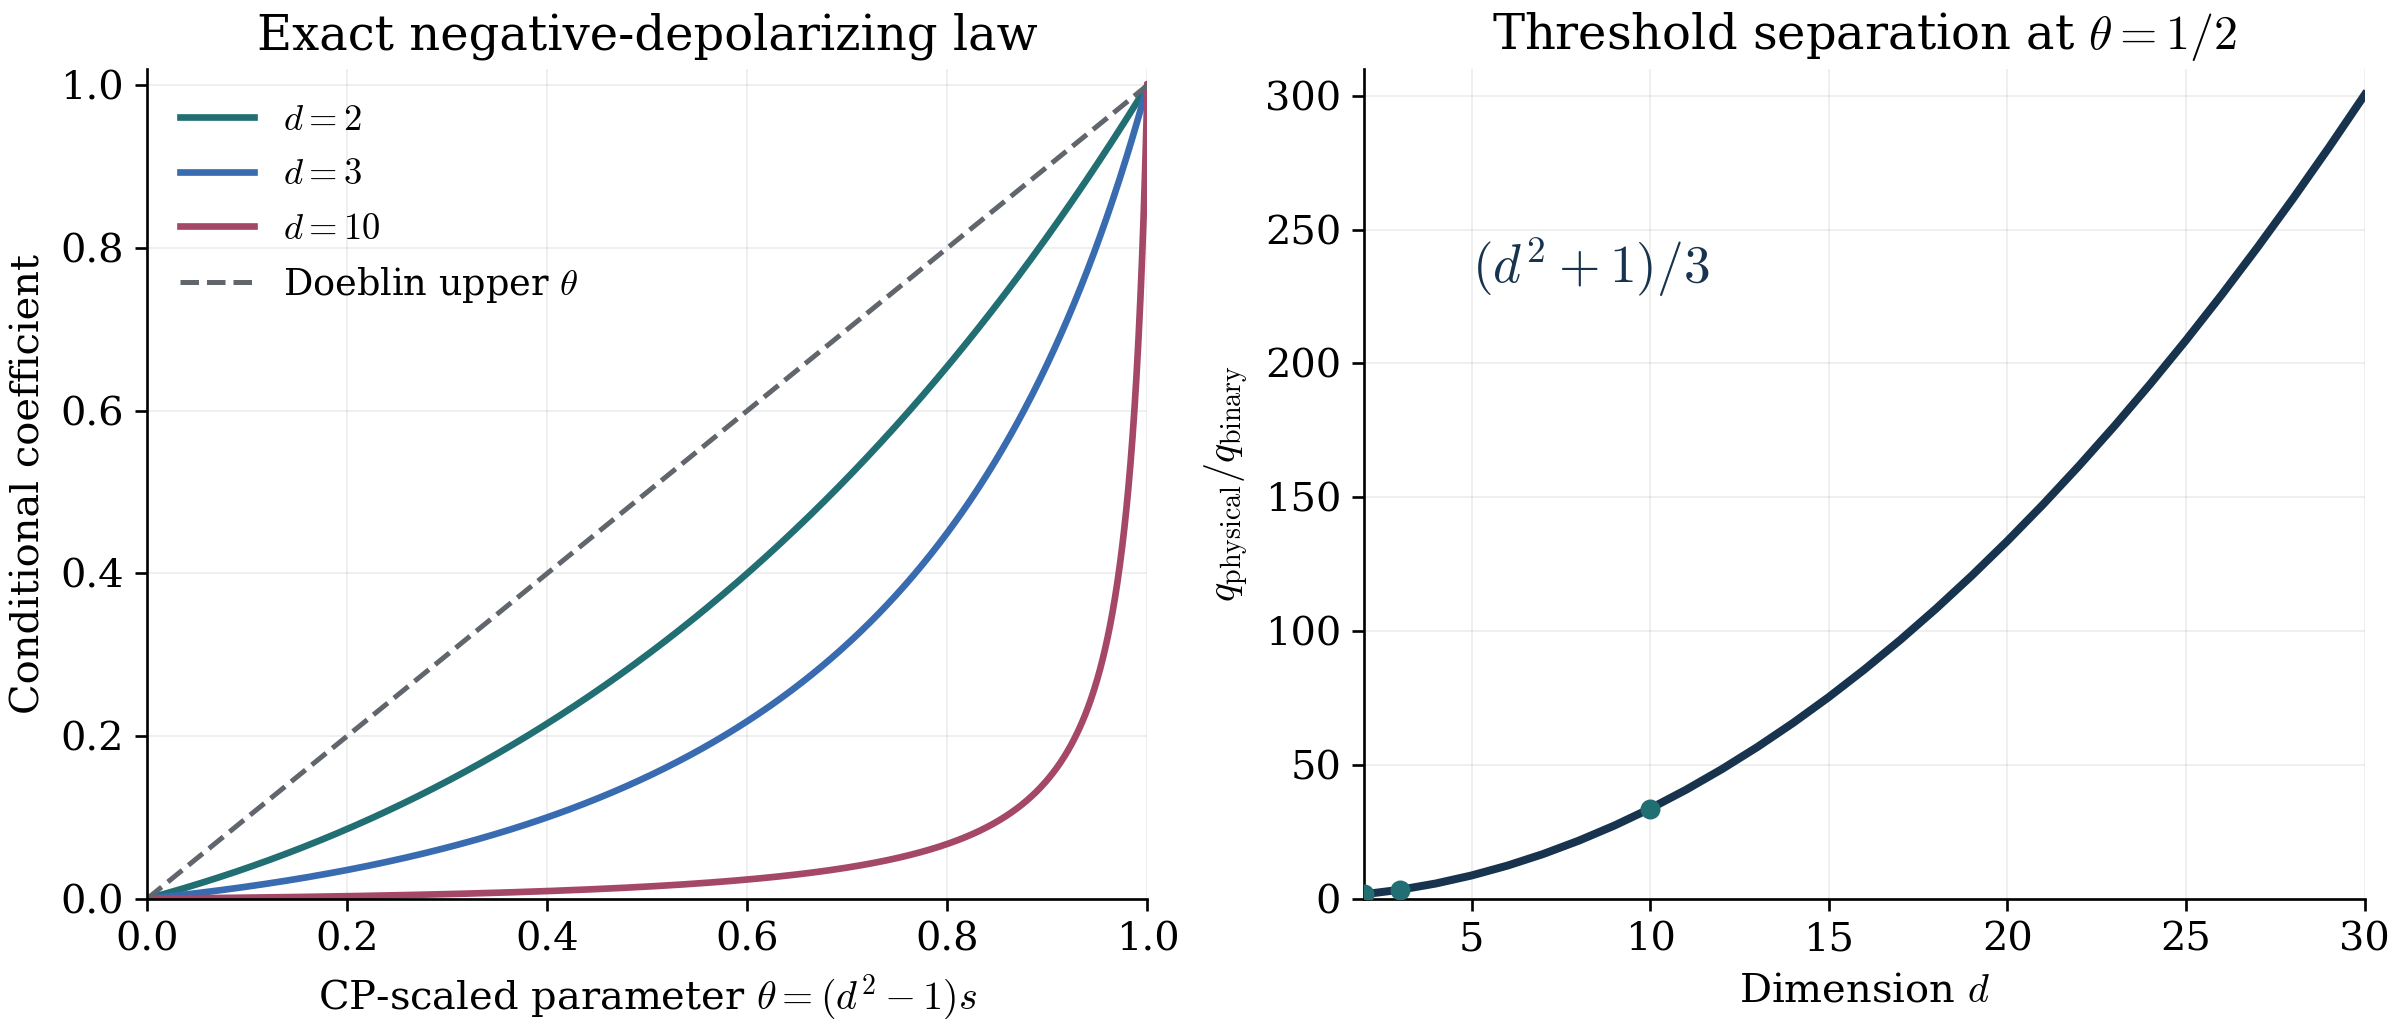
\includegraphics[width=\textwidth]{exact_contraction_curves.png}
\caption{Evaluations of the exact formulas. Left: conditional contraction across the physical negative branch, with $\theta=(d^2-1)s$. Right: the ratio of the physical erasure-simulation threshold to the all-reference binary threshold at $\theta=1/2$. The plotted values are consequences of the proofs, not numerical evidence for them.}
\end{figure}

\subsection{An explicit multi-hypothesis witness}
The $n$ equiprobable Bell-complement inputs
\[
 \rho_i=\frac{I_n-\Phi_i}{n-1}
\]
have the same reference marginal $\rho_{i,T}=I_T/d$. Under $\cN_s$ their outputs are
$[(1-b)I+s\Phi_i]/(n-1)$. The Bell projective measurement is optimal: all outputs commute, and for each Bell outcome its own label has the largest posterior weight. Hence
\[
 P_{\rm guess}(\cN_s)=\frac{1+s}{n}.
\]
For the erasure channel, successful transmission gives optimal guessing probability $1/(n-1)$; the erasure branch carries no label information and gives $1/n$. Thus
\[
 P_{\rm guess}(\cE_q)=\frac{n-1+q}{n(n-1)}.
\]
The first exceeds the second exactly when $q<(n-1)s$, detecting the entire failure-of-degradation interval, including the region where every binary reference-assisted test is dominated. This is a concrete consequence of the exact thresholds, not an asserted new general comparison theorem.

\section{Related work and scope}
The closest inspected primary results are separated by their actual optimization domains. The conditional framework and Doeblin upper are prior~\cite{Conditional,Doeblin}. Hiai and Ruskai~\cite{HiaiRuskai} give ordinary unital-qubit trace contraction through the Bloch operator norm; their metric contractions concern another functional and do not subtract an arbitrary unequal reference marginal. Choi and Li~\cite{ChoiLi} supply the standard unital-qubit normal form.

Eriksson's unital-qubit manuscript~\cite{ErikssonUnital} determines equal-reference SLD, quadratic chi-square and triangular Petz quantities through a four-weight harmonic expression. It already contains the qubit--qutrit support geometry used above and dimension-dependent depolarizing Fisher/Petz laws. Its functionals and matching bounds differ from the trace-gap problem here. The common-support manuscript~\cite{ErikssonCQ} is also prior; its simplex/support machinery and qualitative strictness results are credited prior ingredients.

The literature comparison is incomplete and does not establish first priority. The exact classification for the full Pauli family and the dimension-uniform depolarizing theorem are stated independently of that historical question. No claim is made to resolve the general pure-state restriction question, relative-entropy contraction, tensorization, channel capacities, or finite-reference computability for arbitrary channels.

\section{Formal verification and reproducibility}\label{sec:formal}
\textbf{Verification passed on 29 October 2026.}
All 56 included local proof modules were rebuilt from source with zero compiler errors. The final audit checked 42 essential exported declarations; every reported axiom belonged to the standard foundation set specified below. The actual full signed depolarizing-channel constructor and the final concrete Fourier/Bell coefficient theorem are included in this successful build.

The formalization represents a quantum channel as a complex-linear map with proved complete positivity and trace preservation. Density matrices have PSD and trace-one proofs. The trace norm is the sum of absolute values of actual Hermitian eigenvalues. Partial traces are explicit matrix sums, and the coefficient is a real supremum of actual positive-denominator ratios over all finite references. The code proves the channels, witnesses, normalization, norm bounds, ratio membership, limiting passage and matching upper; a scalar identity alone is not treated as verification of a contraction theorem.

The pinned environment is Lean 4.19.0 with Mathlib commit
\begin{center}\small\ttfamily c44e0c8ee63ca166450922a373c7409c5d26b00b\end{center}
The verifier deletes local proof object files, rebuilds every included local source with \path{--trust=0 -j1 -DwarningAsError=true}, checks the pinned dependency checkout and source hashes, and inspects the transitive axiom dependencies of the essential exported statements. Its allowed standard foundations are propositional extensionality, classical choice and quotient soundness. No added mathematical axioms or unfinished proof holes are permitted.

The public-facing theorem files are the Pauli exact-law module, the final depolarizing exact-law module, the positive-branch module and the comparison modules. Intermediate Bell, frame, scalar and effect modules are included as source, with their actual dependencies. The supplied verification record and theorem audit identify the checked source hashes, module count and exported statements.

To reproduce with the pinned project, install its Lean toolchain, obtain the matching Mathlib dependency and cache, then run
\begin{verbatim}
lake exe cache get
python3 verify.py
\end{verbatim}
An existing clean pinned Mathlib checkout can be used with
\begin{verbatim}
python3 verify.py --lean /path/to/lean \
  --mathlib /path/to/pinned/mathlib4
\end{verbatim}
The source package includes no local compiled proof objects. The formal verification certifies the stated mathematics in its definitions; it does not establish novelty, significance, peer review, or correspondence of every additional prose corollary to a separate formal theorem.

\begin{thebibliography}{9}
\bibitem{Conditional} C. Hirche, I. George, T. Nuradha and M. M. Wilde.
\emph{Conditional contraction coefficients and their applications to quantum networks.}
2026, arXiv:2608.27171v1. \url{https://arxiv.org/abs/2608.27171v1}.
\bibitem{Doeblin} I. George, C. Hirche, T. Nuradha and M. M. Wilde.
\emph{Quantum Doeblin Coefficients: Interpretations and Applications.}
2026 version, arXiv:2503.22823v3. \url{https://arxiv.org/abs/2503.22823v3}.
\bibitem{ChoiLi} M.-D. Choi and C.-K. Li.
\emph{On unital qubit channels.} Quantum Information and Computation 23 (2023), 562--576.
\url{https://arxiv.org/abs/2301.01358}.
\bibitem{HiaiRuskai} F. Hiai and M. B. Ruskai.
\emph{Contraction coefficients for noisy quantum channels.} Journal of Mathematical Physics 57 (2016), 015211.
\url{https://arxiv.org/abs/1508.03551}.
\bibitem{ErikssonUnital} L. Eriksson.
\emph{Complete contraction of unital qubit channels and order-constrained depolarization.}
AIRR working paper ARR-2026-77DGRYDGXD8MDSY2-v4, 27 October 2026.
\url{https://airr.science/papers/ARR-2026-77DGRYDGXD8MDSY2/versions/v4/}.
\bibitem{ErikssonCQ} L. Eriksson.
\emph{Common support and complete contraction with quantum side information.}
AIRR working paper ARR-2026-564FZ70CSN83KACD-v3, 28 October 2026.
\url{https://airr.science/papers/ARR-2026-564FZ70CSN83KACD/versions/v3/}.
\bibitem{Jencova} A. Jen\v{c}ov\'a.
\emph{Comparison of quantum channels and statistical experiments.}
2015 preprint, revised 2016, arXiv:1512.07016v2. \url{https://arxiv.org/abs/1512.07016v2}.
\end{thebibliography}
\end{document}
